\documentclass[pdf,9pt,xcolor=dvipsnames,hide notes]{beamer}\usepackage[]{graphicx}\usepackage[]{color}
%% maxwidth is the original width if it is less than linewidth
%% otherwise use linewidth (to make sure the graphics do not exceed the margin)
\makeatletter
\def\maxwidth{ %
  \ifdim\Gin@nat@width>\linewidth
    \linewidth
  \else
    \Gin@nat@width
  \fi
}
\makeatother

\definecolor{fgcolor}{rgb}{0.345, 0.345, 0.345}
\newcommand{\hlnum}[1]{\textcolor[rgb]{0.686,0.059,0.569}{#1}}%
\newcommand{\hlstr}[1]{\textcolor[rgb]{0.192,0.494,0.8}{#1}}%
\newcommand{\hlcom}[1]{\textcolor[rgb]{0.678,0.584,0.686}{\textit{#1}}}%
\newcommand{\hlopt}[1]{\textcolor[rgb]{0,0,0}{#1}}%
\newcommand{\hlstd}[1]{\textcolor[rgb]{0.345,0.345,0.345}{#1}}%
\newcommand{\hlkwa}[1]{\textcolor[rgb]{0.161,0.373,0.58}{\textbf{#1}}}%
\newcommand{\hlkwb}[1]{\textcolor[rgb]{0.69,0.353,0.396}{#1}}%
\newcommand{\hlkwc}[1]{\textcolor[rgb]{0.333,0.667,0.333}{#1}}%
\newcommand{\hlkwd}[1]{\textcolor[rgb]{0.737,0.353,0.396}{\textbf{#1}}}%
\let\hlipl\hlkwb

\usepackage{framed}
\makeatletter
\newenvironment{kframe}{%
 \def\at@end@of@kframe{}%
 \ifinner\ifhmode%
  \def\at@end@of@kframe{\end{minipage}}%
  \begin{minipage}{\columnwidth}%
 \fi\fi%
 \def\FrameCommand##1{\hskip\@totalleftmargin \hskip-\fboxsep
 \colorbox{shadecolor}{##1}\hskip-\fboxsep
     % There is no \\@totalrightmargin, so:
     \hskip-\linewidth \hskip-\@totalleftmargin \hskip\columnwidth}%
 \MakeFramed {\advance\hsize-\width
   \@totalleftmargin\z@ \linewidth\hsize
   \@setminipage}}%
 {\par\unskip\endMakeFramed%
 \at@end@of@kframe}
\makeatother

\definecolor{shadecolor}{rgb}{.97, .97, .97}
\definecolor{messagecolor}{rgb}{0, 0, 0}
\definecolor{warningcolor}{rgb}{1, 0, 1}
\definecolor{errorcolor}{rgb}{1, 0, 0}
\newenvironment{knitrout}{}{} % an empty environment to be redefined in TeX

\usepackage{alltt}

%%%%%%%%%%%%%%%%%%%%%%%%%%% 
%%%%%      TEMA      %%%%%%
%%%%%%%%%%%%%%%%%%%%%%%%%%%
\usetheme{Rochester}                       % tema
\usecolortheme{orchid}                    % cores
\usefonttheme[onlymath]{serif}            % fonte modo matematico

%%%%%%%%%%%%%%%%%%%%%%%%%%% 
%%%%%    PACOTES      %%%%%
%%%%%%%%%%%%%%%%%%%%%%%%%%%

% \usepackage[alf]{abntex2cite}             % citações no padrão ABNT
% \usepackage[brazil]{babel}                % idioma
\usepackage{Sweave}                       % Sweave
\usepackage{color}                        % controle das cores
\usepackage[T1]{fontenc}                  % codificacao de fontes
\usepackage{graphicx}                     % inclusão de gráficos
\usepackage[utf8]{inputenc}               % codificacao de caracteres
\usepackage{lmodern}
\usepackage{array}
\usepackage{multirow}
\usepackage{enumerate}                    % índices numéricos 
\usepackage{footnote}                     % Lidar com notas de rodapé
\usepackage{booktabs}                     % Tabelas com qualidade de publicação diversas situações
\usepackage{hyperref}                     % para citar hyperlinks da web
\usepackage{adjustbox}
\usepackage{caption}
\newcommand\fnote[1]{\captionsetup{font=small}\caption*{#1}}

%%%%%%%%%%%%%%%%%%%%%%%%%%% 
%%%   INF. DOCUMENTO    %%%
%%%%%%%%%%%%%%%%%%%%%%%%%%%

\title[UFRGS]{Introdução}
\author[Estatística Geral II]{Fernando B. Sabino da Silva}

\date{05/03/18}
\IfFileExists{upquote.sty}{\usepackage{upquote}}{}
\begin{document}
%\SweaveOpts{concordance=TRUE}

%%%%%%%%%%%%%%%%%%%%%%%%%%% 
%%%%%     SUMÁRIO     %%%%%
%%%%%%%%%%%%%%%%%%%%%%%%%%%

\begin{frame}
   \titlepage
\end{frame}

\begin{frame}[plain]\frametitle{Sumário}
%\small\tableofcontents
\tableofcontents
\end{frame}

%%%
% OBJETIVOS
%%%

\section{Objetivos}

\begin{frame}\frametitle{Objetivos}
Ao final desta aula os alunos deverão ser capazes de:
  \begin{itemize}
    \item Conhecer alguns campos de atuação da Econometria e sua relação com a teoria econômica;
    \item Diferir sobre Modelos Econômicos e Modelos Econométricos;
    \item Entender o papel dos dados na definição do método econométrico a ser utilizado;
    \item Entender conceitos de Ciência de Dados e sua relação com a Econometria;
    \item Conhecer a plataforma DataCamp que será usada para aprendizagem da linguagem R.
  \end{itemize}
\end{frame}

%%%
% INTRODUÇÃO
%%%

\section{Introdução}

\subsection{Econometria e Teoria Econômica}
\begin{frame}\frametitle{Econometria e Teoria Econômica}
  \begin{itemize}
    \item Por meio da Econometria é possível avaliar empiricamente a teoria econômica:
    \begin{itemize}
      \item Explicar fatos passados;
      \item Testar teorias e hipóteses;
      \item Prever resultados de políticas ou eventos futuros;
      \item Estimar relações entre variáveis econômicas.
    \end{itemize}
    \item Isso é viável porque, em geral, \textbf{há relações de equilíbrio de longo prazo} entre variáveis econômicas.
  \end{itemize}
  \begin{itemize}
    \item O economista pode fazer uso de diversos campos da econometria de acordo com o \textbf{fundamento econômico}:
    \begin{itemize}
      \item Econometria básica (regressão linear múltipla, classificação...)
      \item Econometria usando Séries Temporais (ARIMA, GARCH, MIDAS, VAR, VEC, ...)
      \item Econometria Não Paramétrica (Estimação de Densidades e Regresões não paramétricas, ...)
      \item Microeconometria (Dados em painel, ...)
      \item Macroeconometria (DSGE, DSGE-VAR, ...)
    \end{itemize}
  \end{itemize}
\end{frame}


\subsection{Modelo Econômico}
\begin{frame}\frametitle{Modelo Econômico}
Quais os efeitos do \textbf{treinamento} sobre a \textbf{produtividade} do trabalhador?
\begin{equation}
salárioh = f\left( educ, exper, treina \right)
\end{equation}

onde: 
  \begin{itemize}
    \item $salárioh$ é o salário-hora;
    \item $educ$ representa os anos de educação formal;
    \item $exper$ refere-se aos de experiência no mercado de trabalho;
    \item $treina$ corresponde as semanas ocupadas em treinamento.\\~\\
  \end{itemize}

\textbf{Hipótese:} Os trabalhadores são pagos de acordo com sua produtividade.
\end{frame}

\subsection{Modelo Econométrico}
\begin{frame}\frametitle{Modelo Econométrico} 
Um modelo econométrico para o exemplo anterior
\begin{equation}
salárioh ={\beta}_{0}+{\beta}_{1}educ+{\beta}_{2}exper+{\beta}_{3}treina+u
\end{equation}

onde termo $u$ contém todos os outros fatores não incluídos na equação (sejam observados diretamente ou não), mas que podem influenciar a produtividade, tais como:
  \begin{itemize}
    \item aptidão inata;
    \item qualidade da educação;
    \item formação da família.\\~\\
  \end{itemize}
\textbf{Objetivo:} Testar hipótese sobre o parâmetro ${\beta}_{3}$. Exemplo: O efeito marginal é diferente de zero?
\end{frame}


\subsection{Ciência de Dados}
\subsubsection{Definição}
\begin{frame}\frametitle{Definição} 
  \begin{itemize}
    \item Com a migração para a internet, produzimos um fluxo constante e exaustivo de informação digital;
    \item Estima-se que \textbf{90\% dos dados armazenados no mundo} foram produzidos apenas nos \textbf{últimos dois anos};
    \item Informação tornou-se a moeda mais poderosa e exige que o mercado saiba interpretá-la a seu favor;
    \item Logo, a profissão do Cientista de Dados se torna crucial;
    \item Áreas de atuação: varejo, saúde, finanças, telecomunicações, segurança, transporte, economia, recursos humanos, ...\\~\\
  \end{itemize}
\textbf{Definição 1}: Ciência de Dados é o termo usado para o processo de extrair \emph{insigths (valor)} de dados que são coletados de várias fontes (estruturados e não estruturados) \\~\\
\textbf{Definição 2}: Consiste de um conjunto de especialidades, tais como estatística, matemática, programação, computação e \emph{business}
\begin{itemize}
\item Leia mais em \url{http://datascience.columbia.edu/data-for-good-preface}
\end{itemize}

\end{frame}

\subsubsection{Dados e Tomada de Decisão}
\begin{frame}\frametitle{Dados e Tomada de Decisão} 
\textbf{Exemplo}: Recrutamento Interno de Colaboradores \\~\\
  \begin{itemize}
    \item \textbf{O que?:} Construir algoritmo que recomende colaboradores internos e/ou em processo de desligamento com maior probabilidade de performar bem nas vagas disponíveis considerando as restrições de negócio e exigências das vagas.
    \item \textbf{Por quê?:} Auxiliar instituição financeira em gestão de pessoas por meio da redução do turnover (em média 7.000 pessoas/ano) e, consequentemente, minimização dos seguintes custos médios por colaborador:
    \begin{itemize}
      \item Desligamento: R\$ 48.443,91
      \item Contratação: R\$ 4.458,00
      \item Trabalhista: R\$ 93.810,54 \\~\\
    \end{itemize}
  \end{itemize}
\textbf{Custo Total no Ano}: R\$ 1.026.987.150,00
\end{frame}

\subsubsection{O Processo de Ciência de Dados}
\begin{frame}\frametitle{O Processo de Ciência de Dados} 
  \begin{enumerate}
    \item Identificar o problema da área de negócio;
    \item Compreender o problema (entidades e atributos);
    \begin{itemize} 
        \item Exemplos de entidades: Cliente, Produto, Contrato, Vendas, etc.
        \item Exemplos de atributos: Código do Produto (Entidade Produto), Nome do Cliente (Entidade Cliente).
     \end{itemize} 
    \item Coletar conjuntos de dados que representem as entidades;
    \item Limpar e transformar os dados;
    \item Compreender os relacionamentos entre os dados;
    \item Criar modelos estatísticos e matemáticos que representem os relacionamentos;
    \item Utilizar os modelos para fazer predições;
    \item Entregar valor e resultado.
  \end{enumerate}
\end{frame}

\subsection{Big Data}
\subsubsection{Dados Gerados por Minuto}
\begin{frame}\frametitle{Dados Gerados por Minuto} 
  \begin{figure}[hb]
    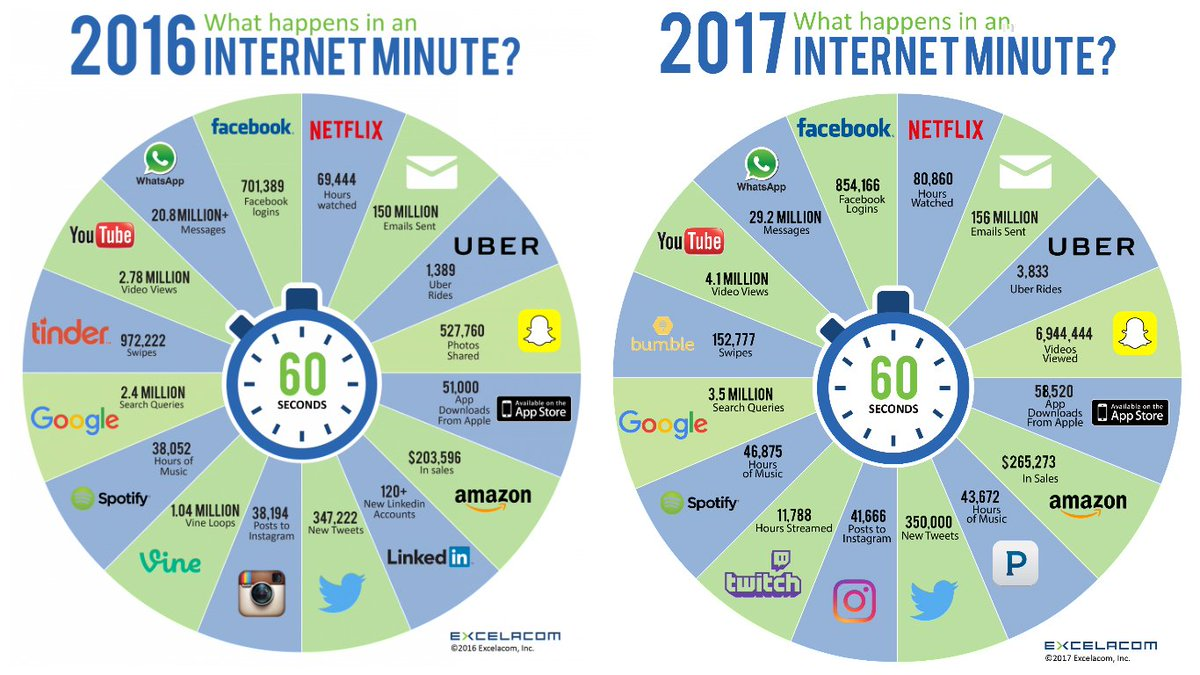
\includegraphics[width=3.5in]{Figure/dataGeneratorByMinuteExcelacom.jpg}
  \end{figure}
\end{frame}

\subsubsection{Velocidade de Crescimento dos Dados}
\begin{frame}\frametitle{Velocidade de Crescimento dos Dados} 
  \begin{figure}[hb]
    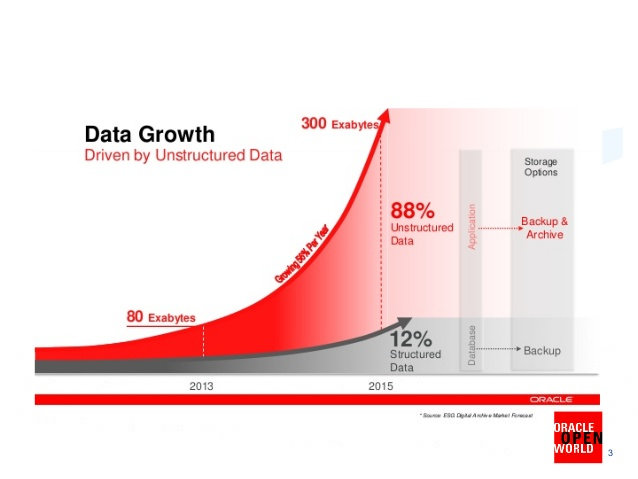
\includegraphics[width=3.5in]{Figure/dataGrowth.jpg}
  \end{figure}
\end{frame}

%%%
% Aplicação Prática
%%%

% \section{Exemplo Prático}
% 
% \subsection{Turnover de Colaboradores}
% \begin{frame}\frametitle{Turnover de Colaboradores}
% \end{frame}

\end{document}
